% Background

\chapter{Background} % Main chapter title

\label{chapter2_bg}
This chapter presents some background for the content of this thesis.

\section{Models and Model Driven Software Development}
\label{mdsd}
Software development is a complex and difficult task that requires the investment of significant resources and carries major risk of failure. According to its proponents, model-driven (MD) software development approaches are improving the way we build software. Model-driven approaches putatively increase developer productivity, decrease the cost (in time and money) of software construction, improve software reusability, and make software more maintainable. Likewise, model-driven techniques promise to aid in the early detection of defects such as design flaws, omissions, and misunderstandings between clients and developers. \par
	If a model is a representation of a system, then in some sense, programming in any language involves some kind of model. Whether we explicitly create artifacts we call models—especially conceptual models—or whether we implicitly map between our internal mental models of the world and the systems we produce, we are nonetheless involved in a modeling process as we construct software. And so MD is more about raising the level of abstraction of our programming models rather than introducing models into the process in the first place. Models  help software engineers communicate more effectively with the many stakeholders who need to participate in the software development process. Improved communication leads to increased understanding, more reasonable expectations, and a better overall work product. Models also let programmers visualize the finished product without requiring its full construction first. By examining the model we can discover design flaws that are far less expensive to resolve up-front rather than after construction has begun (or worse, been completed).\par
	Model-driven software development~\cite{liddle2011model} is a software design approach for the development of software systems. It provides a set of guidelines for the structuring of specifications, which are expressed as models. Model-driven architecture is a kind of domain engineering, and supports model-driven engineering of software systems.\par
	The three primary goals of MDA are portability, interoperability, and reusability, and the key abstraction for delivering on these goals is architectural separation of concerns. MDA describes three main layers of architectural abstraction, called viewpoints: computation independent, platform independent, and platform specific. MDA describes systems using models that correspond to the three viewpoints. A computation independent model (CIM) describes a system environment and its requirements using terminology that is familiar to practitioners in the system domain. A platform independent model (PIM) describes a system’s structure and functions formally, and yet without specifying platform-specific implementation details. At the lowest level of the MDA architecture, a platform specific model (PSM) includes details that are important to the implementation of a system on a given platform.


\section{Data Access Object}
\label{dao}
In computer software, a data access object (DAO)~\cite{DAO} is an object that provides an abstract interface to some type of database or other persistence mechanism. By mapping application calls to the persistence layer, the DAO provides some specific data operations without exposing details of the database. This isolation supports the Single responsibility principle. It separates what data access the application needs, in terms of domain-specific objects and data types (the public interface of the DAO), from how these needs can be satisfied with a specific DBMS or database schema. Because the interface exposed by the DAO to clients does not change when the underlying data source implementation changes, this pattern allows the DAO to adapt to different storage schemes without affecting its clients or business components. Essentially, the DAO acts as an adapter between the component and the data source.

\section{Access Control List}
\label{acl}
An Access Control List (ACL)~\cite{shirey2007internet} is a mechanism that implements access control for a system resource by enumerating the system 	entities that are permitted to access the resource and stating, either implicitly or explicitly, the access modes granted to each entity. A filesystem ACL is a data structure (usually a table) containing entries that specify individual user or group rights to specific system objects such as programs, processes, or files. The privileges or permissions determine specific access rights, such as whether a user can read from, write to, or execute an object. +Role,Permission

\section{HTTP}
The Hypertext Transfer Protocol (HTTP)~\cite{fielding2006hypertext} is an application-level protocol for distributed, collaborative, hypermedia information systems. HTTP has been in use by the World-Wide Web global information initiative since 1990. HTTP functions as a request–response protocol in the client–server computing model. A web browser, for example, may be the client and an application running on a computer hosting a website may be the server. The client submits an HTTP request message to the server. The server, which provides resources such as HTML files and other content, or performs other functions on behalf of the client, returns a response message to the client. The response contains completion status information about the request and may also contain requested content in its message body. HTTP resources are identified and located on the network by Uniform Resource Locators (URLs), using the Uniform Resource Identifiers (URI's) schemes http and https. URIs and hyperlinks in HTML documents form inter-linked hypertext documents.




\subsection{HTTP session}
An HTTP session is a sequence of network request-response transactions. An HTTP client initiates a request by establishing a Transmission Control Protocol (TCP) connection to a particular port on a server (typically port 80, occasionally port 8080; see List of TCP and UDP port numbers). An HTTP server listening on that port waits for a client's request message. Upon receiving the request, the server sends back a status line, such as "HTTP/1.1 200 OK", and a message of its own. The body of this message is typically the requested resource, although an error message or other information may also be returned.




\subsection{Request methods}
HTTP defines methods to indicate the desired action to be performed on the identified resource. What this resource represents, whether pre-existing data or data that is generated dynamically, depends on the implementation of the server. The most common methods which are used in this thesis are presented below.

\paragraph{GET}
The GET method requests a representation of the specified resource. Requests using GET should only retrieve data and should have no other effect. The W3C has published guidance principles on this distinction, saying, "Web application design should be informed by the above principles, but also by the relevant limitations.

\paragraph{POST}
The POST method requests that the server accept the entity enclosed in the request as a new subordinate of the web resource identified by the URI. The data POSTed might be, for example, an annotation for existing resources; a message for a bulletin board, newsgroup, mailing list, or comment thread; a block of data that is the result of submitting a web form to a data-handling process; or an item to add to a database.

\paragraph{PUT}
The PUT method requests that the enclosed entity be stored under the supplied URI. If the URI refers to an already existing resource, it is modified; if the URI does not point to an existing resource, then the server can create the resource with that URI.

\paragraph{DELETE}
The DELETE method deletes the specified resource.




\subsection{Status Codes}
In HTTP/1.0 and since, the first line of the HTTP response is called the status line and includes a numeric status code (such as "404") and a textual reason phrase (such as "Not Found"). The way the user agent handles the response primarily depends on the code and secondarily on the other response header fields. Custom status codes can be used since, if the user agent encounters a code it does not recognize, it can use the first digit of the code to determine the general class of the response. HTTP status code is primarily divided into five groups for better explanation of request and responses between client and server, and are presented below. 

\paragraph{1xx Informational responses}
An informational response indicates that the request was received and understood. It is issued on a provisional basis while request processing continues. It alerts the client to wait for a final response. The message consists only of the status line and optional header fields, and is terminated by an empty line.

\paragraph{2xx Success}
This class of status codes indicates the action requested by the client was received, understood, accepted, and processed successfully.

\paragraph{3xx Redirection}
This class of status code indicates the client must take additional action to complete the request. Many of these status codes are used in URL redirection.[2]
A user agent may carry out the additional action with no user interaction only if the method used in the second request is GET or HEAD. A user agent may automatically redirect a request. A user agent should detect and intervene to prevent cyclical redirects.

\paragraph{4xx Client errors}
This class of status code is intended for situations in which the client seems to have errored. Except when responding to a HEAD request, the server should include an entity containing an explanation of the error situation, and whether it is a temporary or permanent condition. These status codes are applicable to any request method. User agents should display any included entity to the user.

\paragraph{5xx Server errors}
The server failed to fulfill an apparently valid request. Response status codes beginning with the digit "5" indicate cases in which the server is aware that it has encountered an error or is otherwise incapable of performing the request. Except when responding to a HEAD request, the server should include an entity containing an explanation of the error situation, and indicate whether it is a temporary or permanent condition. Likewise, user agents should display any included entity to the user. These response codes are applicable to any request method.




\section{REST}
\label{rest}
Representational state transfer (REST)~\cite{w3c2004web} or RESTful web services is a way of providing interoperability between computer systems on the Internet. REST-compliant Web services allow requesting systems to access and manipulate textual representations of Web resources using a uniform and predefined set of stateless operations.  In a RESTful Web service, requests made to a resource's URI will elicit a response that may be in XML, HTML, JSON or some other defined format. The response may confirm that some alteration has been made to the stored resource, and it may provide hypertext links to other related resources or collections of resources. The term is intended to evoke an image of how a well-designed Web application behaves: it is a network of Web resources (a virtual state-machine) where the user progresses through the application by selecting links, such as /user/tom, and operations such as GET or DELETE (state transitions), resulting in the next resource (representing the next state of the application) being transferred to the user for their use. There are six guiding constraints that define a RESTful system.These constraints restrict the ways that the server may process and respond to client requests so that, by operating within these constraints, the service gains desirable non-functional properties, such as performance, scalability, simplicity, modifiability, visibility, portability, and reliability. If a service violates any of the required constraints, it cannot be considered RESTful. The formal REST constraints are represented below.

\subsection{Client-server architecture}
The first constraints added to our hybrid style are those of the client-server architectural style. Separation of concerns is the principle behind the client-server constraints. By separating the user interface concerns from the data storage concerns, we improve the portability of the user interface across multiple platforms and improve scalability by simplifying the server components. Perhaps most significant to the Web, however, is that the separation allows the components to evolve independently, thus supporting the Internet-scale requirement of multiple organizational domains.

\paragraph{Statelessness}
The client–server communication is constrained by no client context being stored on the server between requests. Each request from any client contains all the information necessary to service the request, and session state is held in the client. The session state can be transferred by the server to another service such as a database to maintain a persistent state for a period and allow authentication. The client begins sending requests when it is ready to make the transition to a new state. While one or more requests are outstanding, the client is considered to be in transition. The representation of each application state contains links that may be used the next time the client chooses to initiate a new state-transition.

\paragraph{Cacheability}
As on the World Wide Web, clients and intermediaries can cache responses. Responses must therefore, implicitly or explicitly, define themselves as cacheable or not to prevent clients from reusing stale or inappropriate data in response to further requests. Well-managed caching partially or completely eliminates some client–server interactions, further improving scalability and performance.

\paragraph{Layered system}
A client cannot ordinarily tell whether it is connected directly to the end server, or to an intermediary along the way. Intermediary servers may improve system scalability by enabling load balancing and by providing shared caches. They may also enforce security policies.

\paragraph{Uniform interface}
The uniform interface constraint is fundamental to the design of any REST service. It simplifies and decouples the architecture, which enables each part to evolve independently.





\section{Application Programming Interface}
In computer programming, an Application Programming Interface (API) is a set of subroutine definitions, protocols, and tools for building application software. In general terms, it is a set of clearly defined methods of communication between various software components. A good API makes it easier to develop a computer program by providing all the building blocks, which are then put together by the programmer. An API may be for a web-based system, operating system, database system, computer hardware or software library. An API specification can take many forms, but often includes specifications for routines, data structures, object classes, variables or remote calls. API uses are listed below.

\paragraph{Libraries and Frameworks}
An API is usually related to a software library. The API describes and prescribes the expected behavior (a specification) while the library is an actual implementation of this set of rules. A single API can have multiple implementations (or none, being abstract) in the form of different libraries that share the same programming interface. The separation of the API from its implementation can allow programs written in one language to use a library written in another. 

\paragraph{Operating systems}
An API can specify the interface between an application and the operating system. POSIX, for example, specifies a set of common APIs that aim to enable an application written for a POSIX conformant operating system to be compiled for another POSIX conformant operating system.

\paragraph{Remote APIs}
Remote APIs allow developers to manipulate remote resources through protocols, specific standards for communication that allow different technologies to work together, regardless of language or platform.


\paragraph{WEB APIs}
Web APIs are the defined interfaces through which interactions happen between an enterprise and applications that use its assets. An API approach is an architectural approach that revolves around providing programmable interfaces to a set of services to different applications serving different types of consumers.When used in the context of web development, an API is typically defined as a set of Hypertext Transfer Protocol (HTTP) request messages, along with a definition of the structure of response messages, which is usually in an Extensible Markup Language (XML) or JavaScript Object Notation (JSON) format.

\section{Three-tier Architecture}
\label{3tierarch}
\begin{figure}
	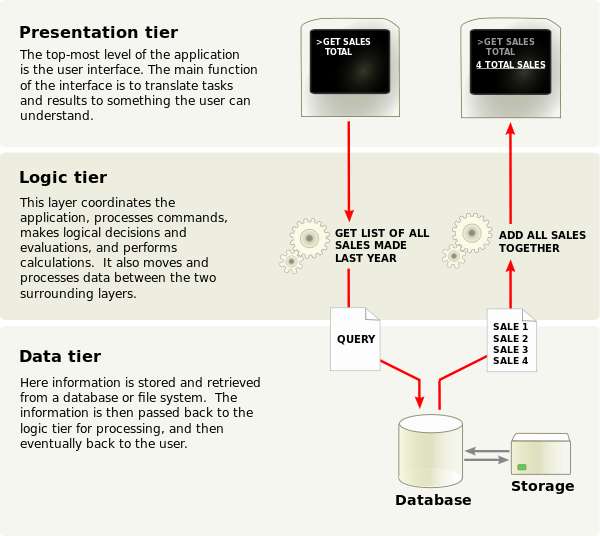
\includegraphics[scale=0.5]{3tier.png}
	\caption{Three-tier Architecture}
	\label{3tier}
\end{figure}

Three-tier architecture~\cite{ramirez2000three} is a client–server software architecture pattern in which the user interface (presentation), functional process logic ("business rules"), computer data storage and data access are developed and maintained as independent modules, most often on separate platforms. Apart from the usual advantages of modular software with well-defined interfaces, the three-tier architecture is intended to allow any of the three tiers to be upgraded or replaced independently in response to changes in requirements or technology. An image of a three-tier architecture can be seen in figure~\ref{3tier}. The three layers are presented below.

\paragraph{Presentation tier}
This is the topmost level of the application. The presentation tier displays information related to such services as browsing merchandise, purchasing and shopping cart contents. It communicates with other tiers by which it puts out the results to the browser/client tier and all other tiers in the network. In simple terms, it is a layer which users can access directly (such as a web page, or an operating system's GUI).

\paragraph{Logic tier}
The logical tier is pulled out from the presentation tier and, as its own layer, it controls an application’s functionality by performing detailed processing.

\paragraph{Data tier}
The data tier includes the data persistence mechanisms (database servers, file shares, etc.) and the data access layer that encapsulates the persistence mechanisms and exposes the data. The data access layer should provide an API to the application tier that exposes methods of managing the stored data without exposing or creating dependencies on the data storage mechanisms. Avoiding dependencies on the storage mechanisms allows for updates or changes without the application tier clients being affected by or even aware of the change.




\section{Single Page Application}
\label{spa}
A single-page application (SPA)~\cite{mikowski2013single} is a web application or web site that fits on a single web page with the goal of providing a user experience similar to that of a desktop application. In an SPA, either all necessary code – HTML, JavaScript, and CSS – is retrieved with a single page load, or the appropriate resources are dynamically loaded and added to the page as necessary, usually in response to user actions. The page does not reload at any point in the process, nor does control transfer to another page, although the location hash or the HTML5 History API can be used to provide the perception and navigability of separate logical pages in the application. Interaction with the single page application often involves dynamic communication with the web server behind the scenes.\par
	There are various techniques available that enable the browser to retain a single page even when the application requires server communication. The most prominent technique currently being used is Ajax. Ajax is a set of Web development techniques using many Web technologies on the client side to create asynchronous Web applications. With Ajax, Web applications can send data to and retrieve from a server asynchronously (in the background) without interfering with the display and behavior of the existing page. By decoupling the data interchange layer from the presentation layer, Ajax allows for Web pages, and by extension Web applications, to change content dynamically without the need to reload the entire page. In practice, modern implementations commonly substitute JSON for XML due to the advantages of being native to JavaScript.



\section{Hierarchical Data Format}
\label{hdf}
\begin{figure}
	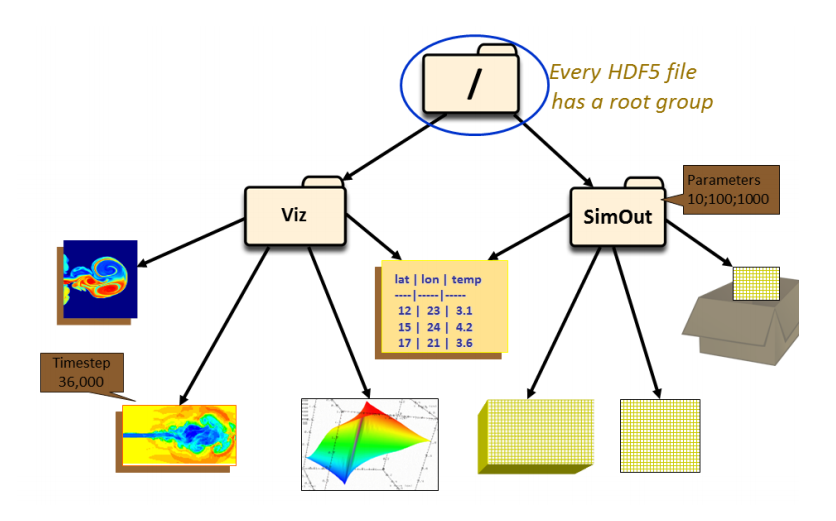
\includegraphics[scale=0.4]{hdf.png}
	\caption{The contents of an HDF file}
	\label{hdf}
\end{figure}
\begin{figure}
	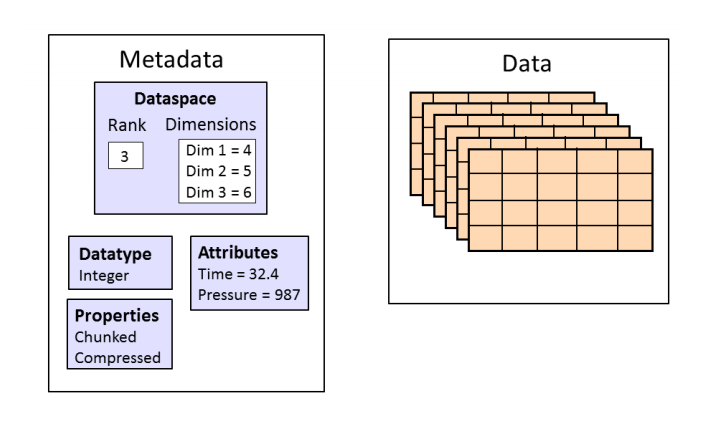
\includegraphics[scale=0.5]{dset.png}
	\caption{The general structure of a dataset}
	\label{dset}
\end{figure}
Hierarchical Data Format (HDF))~\cite{hdf2014hierarchical} is a set of file formats (HDF4, HDF5) designed to store and organize large amounts of data.Many HDF adopters have very large datasets, very fast access requirements, or very complex datasets. Others turn to HDF because it allows them to easily share data across a wide variety of computational platforms using applications written in different programming languages.\par
	HDF allows hierarchical data objects to be expressed in a very natural manner, in contrast to the tables of a relational database.  Whereas relational databases support tables, HDF supports n-dimensional datasets and each element in the dataset may itself be a complex object. Relational databases offer excellent support for queries based on field matching, but are not well-suited for sequentially processing all records in the database or for subsetting the data based on coordinate-style lookup. The contents of an HDF file can be seen in figure~\ref{hdf}.\par
	HDF5 consists of a File Format for storing HDF5 data, a Data Model for logically organizing and accessing HDF5 data from an application, and the Software (libraries, language interfaces, and tools) for working with this format. The data model is described below.
\subsection{Data Model}
The HDF Data Model, also known as the HDF5 Abstract (or Logical) Data Model consists of the building blocks for data organization and specification in HDF5. An HDF5 file (an object in itself) can be thought of as a container (or group) that holds a variety of heterogeneous data objects (or datasets). The datasets can be most anything: images, tables, graphs, or even documents, such as PDF or Excel. The two primary objects in the HDF5 Data Model are described below.

\paragraph{Groups}
HDF5 groups (and links) organize data objects. Every HDF5 file contains a root group that cancontain other groups or be linked to objects in other files. Working with groups and group members is similar in many ways to working with directories and files in UNIX. As with UNIX directories and files, objects in an HDF5 file are often described by giving their full (or absolute) path names.

\paragraph{Datasets}
HDF5 datasets organize and contain the “raw” data values. A dataset consists of metadata that describes the data, in addition to the data itself. Datatypes, dataspaces, properties and (optional) attributes are HDF5 objects that describe a dataset. The datatype describes the individual data elements. The general structure of a dataset can be seen in figure~\ref{dset}.












